
%(BEGIN_QUESTION)
% Copyright 2011, Tony R. Kuphaldt, released under the Creative Commons Attribution License (v 1.0)
% This means you may do almost anything with this work of mine, so long as you give me proper credit

Your task is to sketch a workable PLC program to control the starting and stopping of a conveyor belt, given the following I/O connections and device statuses:

\begin{itemize}
\item{} {\bf Input card channels} 
\item{} {\tt Channel 1} = Start pushbutton (NO) -- {\it pushing this button closes the switch to energize the PLC input}
\item{} {\tt Channel 2} = Stop pushbutton (NC) -- {\it pushing this button opens the switch to de-energize the PLC input}
\item{} {\tt Channel 3} = Speed switch (NO) -- {\it moving conveyor belt closes the switch to energize the PLC input}
\end{itemize}

\begin{itemize}
\item{} {\bf Output card channels} 
\item{} {\tt Channel 1} = Motor contactor -- {\it energizing this PLC output starts the conveyor belt motor}
\end{itemize}

\vskip 10pt

Upon momentarily pushing the ``Start'' button, the conveyor belt motor starts immediately, but will automatically shut down if the belt is not moving within 3 seconds of motor start-up (i.e. a broken or slipping belt condition).  A low speed detected any time after this 3-second ``proof'' period will immediately shut down the conveyor.  Pressing the ``Stop'' button immediately shuts down the conveyor regardless of speed switch status.

$$
\includegraphics[width=15.5cm]{i03550x01.eps}$$

Since you will not have access to PLC programming software during the exam, your address labeling and instruction syntax does not have to be 100\% perfect.  If you can't remember how the exact address is written for channel 3 on card 2 of an Allen-Bradley PLC, for example, or the displayed order of the parameters inside of a Siemens timer instruction, it's no big deal.  All that matters is that your program is clear and unambiguous.  Tagnames (e.g. ``{\tt Start\_switch}'') are recommended in lieu of model-specific address labels such as {\tt I0.6}.

\underbar{file i03550}
%(END_QUESTION)





%(BEGIN_ANSWER)

{\it Half-credit if any important details (e.g. addresses, timer setpoint values) are missing from the sketched program, assuming the basic structure of the program is sound.  No credit should be given for any program failing to properly implement \underbar{all} stated objectives.  If any stated objective will only be implemented inconsistently (rather than reliably, every time), award half-credit.  Deduct 1 point if any gratuitous output bits are used instead of ``internal'' bits.}

\vskip 10pt

Here is one sample program, for Allen-Bradley MicroLogix PLCs:

$$\includegraphics[width=15.5cm]{i03550x02.eps}$$

{\it Award 5 extra-credit points for anyone who includes a reset of the off-delay timer whenever the Stop button is pressed!  This will prevent the conveyor from re-starting if the Stop button is pressed immediately after the Start button is pressed (i.e. if an operator starts the conveyor then changes their mind).}

%(END_ANSWER)





%(BEGIN_NOTES)

{\bf This question is intended for exams only and not worksheets!}.

%(END_NOTES)

